\begin{figure}[h!]
    \begin{center}
    \caption{Effects on Health Infrastructure}\label{fig:11}
    \begin{subfigure}{0.48\textwidth}
        \caption{\scriptsize N. of Municipal Hospitals (per capita*1000)}\label{fig:11a}
        \centering
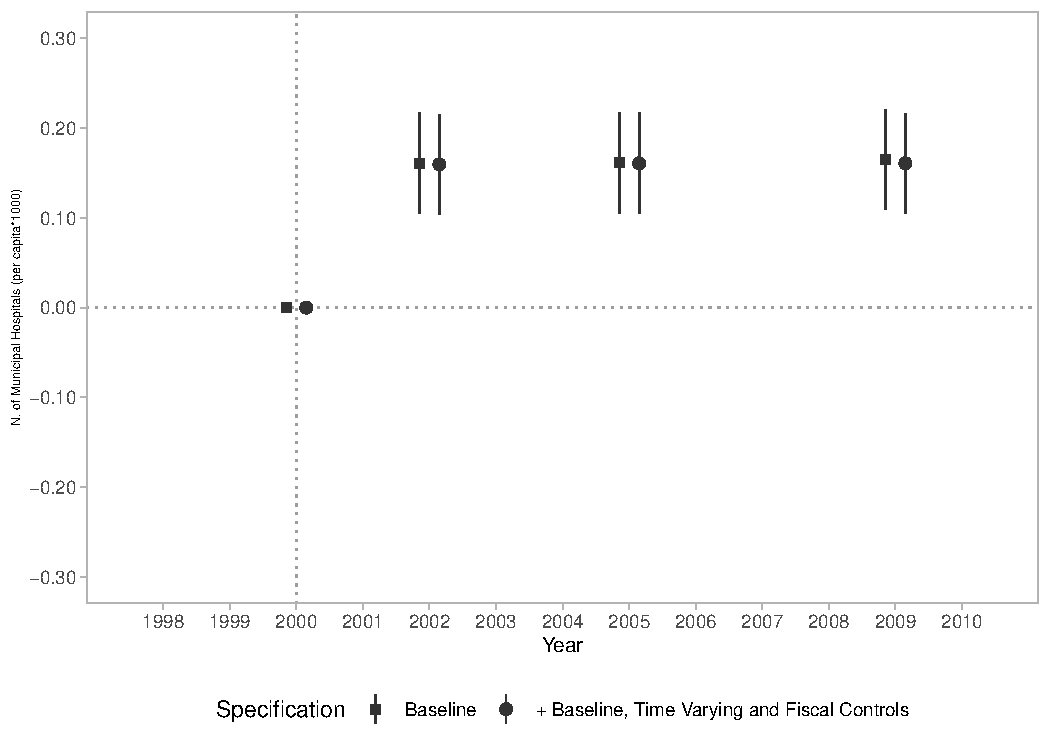
\includegraphics[width=\textwidth]{plots/ams_hospital_mun_pcapita_dist_ec29_baseline_dist_ec29_baseline_11.pdf}
    \end{subfigure}
    \begin{subfigure}{0.48\textwidth}
        \centering
        \caption{\scriptsize N. of Federal and State Hospitals (per capita*1000)}\label{fig:11b}
        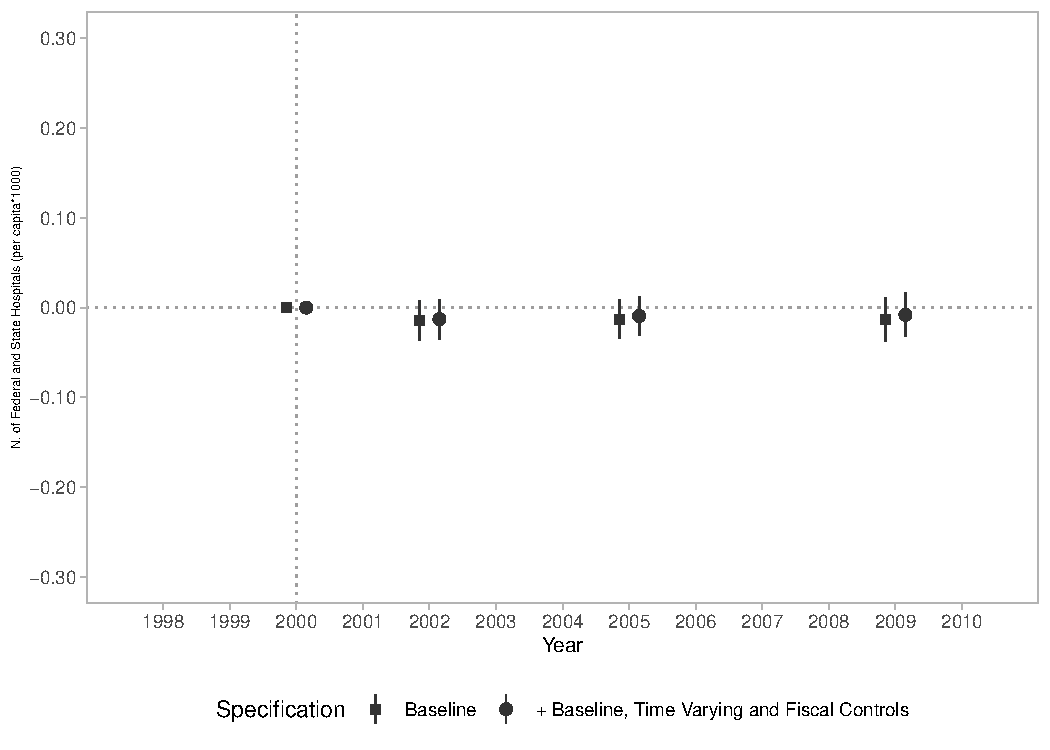
\includegraphics[width=\textwidth]{plots/ams_hospital_nmun_pcapita_dist_ec29_baseline_dist_ec29_baseline_11.pdf}
    \end{subfigure}
    \begin{subfigure}{0.48\textwidth}
        \centering
        \caption{\scriptsize N. of Private Hospitals (per capita*1000)}\label{fig:11c}
        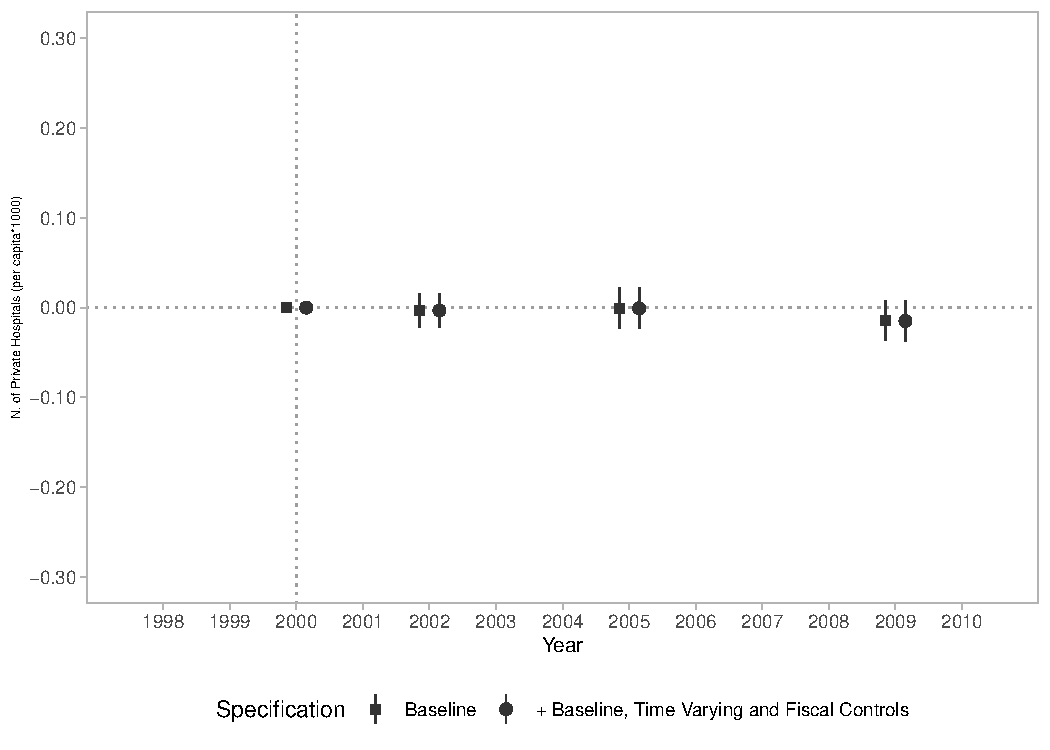
\includegraphics[width=\textwidth]{plots/ams_hospital_pvt_pcapita_dist_ec29_baseline_dist_ec29_baseline_11.pdf}
    \end{subfigure}
    \begin{subfigure}{0.48\textwidth}
        \centering
        \caption{\scriptsize N. of Health Facilities with Ambulatory Service (per capita*1000)}\label{fig:11d}
        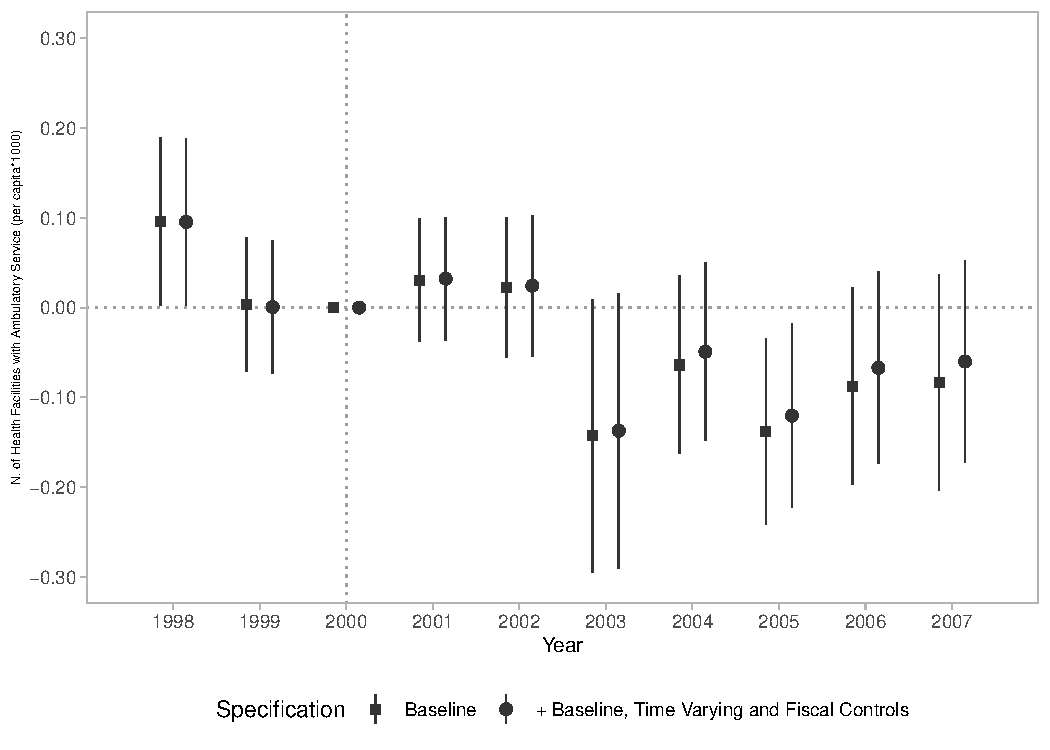
\includegraphics[width=\textwidth]{plots/sia_ncnes_amb_mun_pcapita_dist_ec29_baseline_dist_ec29_baseline_11.pdf}
    \end{subfigure}
    
    \end{center}
    \scriptsize{Notes: The number of observations is 19364 for Figure \ref{fig:11a}, \ref{fig:11b}, \ref{fig:11c} and 48916 for the remaining. DiD Estimates from Equation \ref{eq:2}. Independent variable is the distance to the EC/29 target in p.p. Square dots represent the baseline model with municipality and state-year fixed effects. Round dots represent fully saturated specification (Column 4 in regression Tables). Lines represent 95\% confidence intervals. Arrows, when present, indicate confidence intervals out of the plot bounds. Standard errors are clustered in the municipality level.}
    
\end{figure}